\documentclass{article}
\usepackage[utf8]{inputenc}
\usepackage{graphicx}
\usepackage{fancyvrb}
\usepackage[T1]{fontenc}
\usepackage{lmodern}
\usepackage{hyperref}
\usepackage{xcolor}
\usepackage{verbatim}
\usepackage{amsthm}
\usepackage{amsmath}
\usepackage{caption}
\usepackage{textcomp}
\usepackage{float}

\newcommand{\resource}[1]{(Local copy saved to \texttt{#1})}
\newcommand{\tttilde}[0]{\textasciitilde{}}
\newcommand{\todo}[1]{{\color{blue}{TODO: #1}}}

\theoremstyle{definition}
\newtheorem{program}{Program}
\newtheorem{exercise}{Exercise}

\begin{document}

\section{Background}

This document will develop the concepts of so-called \emph{hybrid parallel programming}, where MPI and OpenMP are both used in the same program in an attempt to gain the benefits of both parallel frameworks. The hybrid parallel programs will be executed on a Raspberry Pi cluster that has already been developed. As such, it is assumed that the previous assignments on building the Pi cluster, executing MPI programs on the cluster, and programming in OpenMP have been covered. In particular, a shared directory is used to run programs on the cluster, which was set up in the MPI cluster assignment.

Recall that OpenMP is a \emph{shared-memory} framework: it is designed to efficiently run parallel programs on a single multi-core computer by allowing the sharing of memory between cores where possible. The basic unit of parallelism in an OpenMP program is a thread, which is relatively lightweight and efficient. On the other hand, MPI is a \emph{distributed-memory} framework: while it has no concept of shared memory, it is capable of running parallel programs across multiple computers simultaneously. The basic unit of parallelism in MPI is a process, which requires more memory than a thread, but two MPI processes on different computers can interact with each other as if they were on the same computer.

In view of this, there is a natural way to combine OpenMP and MPI to run efficient parallel programs across a cluster of computers. We will create exactly one MPI process per computer in the cluster, and use the message passing provided by MPI to communicate between these processes. From within each node's MPI process, we will parallelize that node's work using OpenMP, taking advantage of its lightweight threads and efficient memory sharing capabilities. This approach should thus provide the benefits of both programs.

\section{Hybrid Hello World}

As usual, our first attempt at hybrid parallelism will be a "Hello World" program that prints an identifying message from each thread, provided as \texttt{hybrid-hw.c}. The program is built from features of MPI and OpenMP that we have used before:

\begin{itemize}
    \item This program begins with the call \texttt{MPI\_Init(\&argc, \&argv)} and ends with the call \texttt{MPI\_Finalize()}, as must be the case with every program that uses MPI.
    
    \item The \texttt{MPI\_Comm\_rank} and \texttt{MPI\_Get\_processor\_name} functions are used to compute the MPI process ID and the hostname of the executing MPI process.
    
    \item The \texttt{omp\_get\_thread\_num} function is used to compute the OpenMP thread ID of the executing thread.
    \pagebreak
    \item The \texttt{for} loop is parallelized using the OpenMP compiler directive:
    \begin{verbatim}
#pragma omp parallel for
for (int i = 0; i < 4; i++)\end{verbatim}
    This directive creates separate tasks for each iteration of the loop then distributes each task to a thread as threads are made available to OpenMP, resulting in the parallelization of the loop.
\end{itemize}

Recall that the \texttt{mpicc} compiler should be used to compile an MPI program. However, \texttt{mpicc} is implemented as a \emph{wrapper} around the \texttt{gcc} compiler, in that calling \texttt{mpicc} is ultimately just calling \texttt{gcc} with certain extra command-line arguments that make the MPI library available. Thus we can use the \texttt{-fopenmp} flag to compile our program with OpenMP functionality, just as we have done previously when compiling with \texttt{gcc}.

Once we have compiled our program to an executable, it remains to actually execute it. As before, we will execute our MPI programs using \texttt{mpiexec}. To run the program on multiple nodes in a cluster, we must also pass a hostfile containing the IP addresses of nodes on which to create processes. Since we want to run only one MPI process on each node, our hostfile should contain the IP address of each node only once. 

To correctly use the hostfile, we must pass it to \texttt{mpiexec} with the \texttt{-hostfile} command-line argument. Additionally, the \texttt{-n} argument must be used to tell MPI how many processes to create in total. The following image shows how the program would be compiled and executed on a two-node cluster:

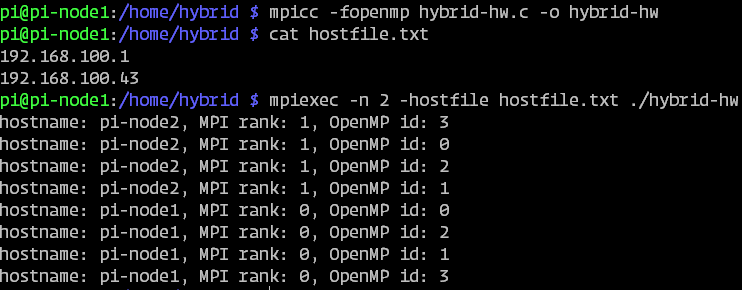
\includegraphics[width=\textwidth]{images/hybrid-hw-output-1.png}

Notice that both nodes print four lines, corresponding to the four iterations of the \texttt{for} loop that each node executes. Since at least four threads are available to OpenMP by default, each iteration of the loop is executed by a different thread, with thread IDs ranging from 0 to 3. Since the MPI process running on each cluster node has its own copy of the program and its own threads, we see that both processes have their own thread with ID 0. Thus, in order to uniquely identify a given thread in our hybrid program, we will need both its MPI rank as well as its OpenMP thread ID.

If we instead explicitly set the available threads to lower than 4, we will see that some OpenMP threads will execute more than one iteration of the loop:

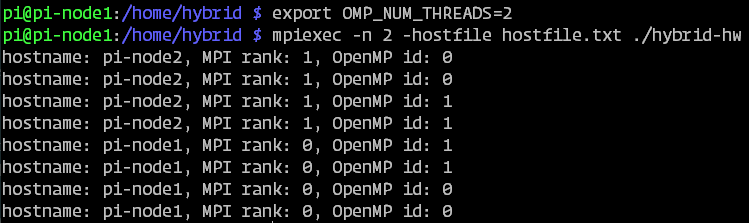
\includegraphics[width=\textwidth]{images/hybrid-hw-output-2.png}

\section{Hybrid prime counting}

This section will revisit the prime counting program that was originally written purely using MPI. We will now modify it to use a hybrid parallel approach. Namely, it will use OpenMP directives to parallelize the work on each individual node, while still using MPI to coordinate the final results of each node. 

When trying to parallelize existing serial code with OpenMP, a natural place to start is to check each of the program's loops to see if their iterations can be easily parallelized. If later loop iterations generally depend on previous iterations, the loop may be difficult to parallelize, but if the loop iterations are mostly independent from each other, then a single OpenMP directive can often be quite effective.

There are two \texttt{for} loops in the original \texttt{primes.c} program that are candidates for parallelization. The first is within the \texttt{is\_prime} function:

\begin{verbatim}
for (int i = 2; i <= sqrt((double)number); i++) {
  if (number % i == 0) return 0;
}
\end{verbatim}

While these loop iterations are indeed independent of each other, each iteration represents a very small amount of work, amounting to essentially only one modulo operation and one numeric comparison. Parallelizing such short iterations can often incur more overhead from scheduling than is worthwhile. The second loop, however, is much more promising:

\begin{verbatim}
int primes_found = 0;
for (int n = a; n <= UPPER_LIMIT; n += k) {
  if (is_prime(n)) primes_found++;
}
\end{verbatim}

This loop body calls \texttt{is\_prime(n)}, which for large \texttt{n} represents enough work to warrant parallelization. However, since the loop iterations write to the external variable \texttt{primes\_found}, we need to take care to update this variable in a thread-safe way. In particular, the following approach \emph{does not work}, since multiple threads may attempt to increment to \texttt{primes\_found} simultaneously, resulting in a race condition:

\begin{verbatim}
// this results in a race condition
#pragma omp parallel for
for (int n = start; n <= end; n++) {
  if (is_prime(n)) primes_found++;
}
\end{verbatim}

There are several ways to fix the above directive to correctly compute \texttt{primes\_found}, but the simplest is to use a sum reduction, a technique we previously used in the parallel selection sort algorithm. With a sum reduction, each thread will maintain its own local copy of \texttt{primes\_found} that isn't vulnerable to a race condition. When the loop ends, the values from each thread will be added serially, resulting in the correct value. The following shows the correct directive that includes the sum reduction:

\begin{verbatim}
#pragma omp parallel for reduction(+:primes_found)
for (int n = start; n <= end; n++) {
  if (is_prime(n)) primes_found++;
}
\end{verbatim}

\begin{exercise}
Compile and execute \texttt{hybrid-primes.c} using one MPI process and four OpenMP threads. You will need to use the \texttt{-lm} command-line argument when compiling, which links the math library containing the \texttt{sqrt} function used by \texttt{is\_prime}. Time the execution using the \texttt{time} utility.

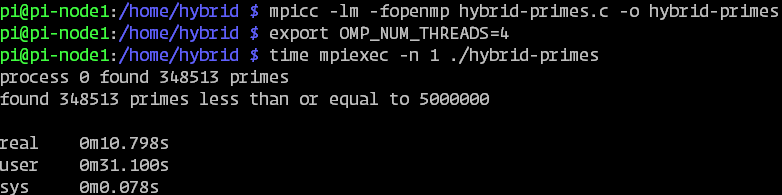
\includegraphics[width=\textwidth]{images/hybrid-primes-output-1.png}
\end{exercise}

\begin{exercise}
\label{ex:primes-2}
Execute \texttt{hybrid-primes} using 1 MPI process for each node in the cluster and 4 OpenMP threads per node.

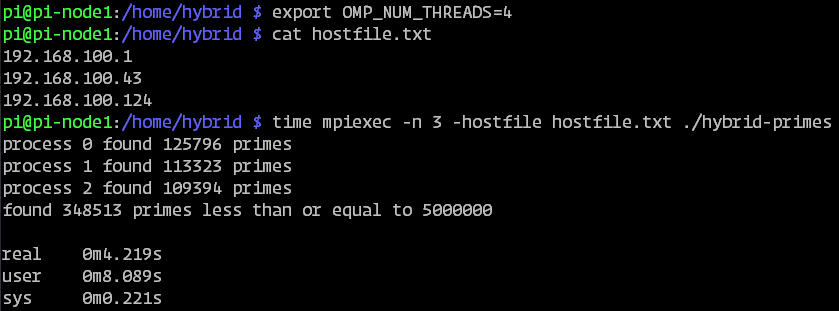
\includegraphics[width=\textwidth]{images/hybrid-primes-output-2.png}
\end{exercise}

\begin{exercise}
Execute \texttt{hybrid-primes} using 4 MPI processes for each node in the cluster and only 1 OpenMP thread per node. Compare the execution time to Exercise \ref{ex:primes-2}.
\end{exercise}

\section{Hybrid matrix multiplication}

This section demonstrates a matrix multiplication program written using hybrid parallel programming. The program is provided as \texttt{hybrid-matmul.c} and is adapted from University of Arizona course materials that are cited at the end of the section.

First, this program allocates \texttt{N}-by-\texttt{N} matrices \texttt{A}, \texttt{B}, and \texttt{C} on the root node (i.e. the node with MPI rank 0). The root node also initializes \texttt{A} and \texttt{B} to have all entries equal to 1. The goal of the program is then to write the matrix product \texttt{AB} into the uninitialized matrix \texttt{C}. The matrix product computation is distributed to all available cluster nodes, each of which computes a \emph{strip} (a number of consecutive rows) of \texttt{C}. MPI message passing is used to coordinate all partial results on the root node, which has the completed result \texttt{C} by the end of the program. Since the input matrices \texttt{A} and \texttt{B} are only initialized on the root node, MPI message passing must be used to send these matrices to non-root nodes as well. 

In order to compute an entry \texttt{C[i][j]} of the matrix product (that is, the entry of \texttt{C} in the \texttt{i}-th row and \texttt{j}-th column), one needs the \texttt{i}-th row of \texttt{A} and the \texttt{j}-th column of \texttt{B}. This follows from the definition of the matrix product:

\begin{verbatim}
C[i][j] = A[i][0]*B[0][j] + A[i][1]*B[1][j] + ... + A[i][N]*B[N][j];
\end{verbatim}

From this, we can deduce that the entirety of \texttt{B} is needed to compute the \texttt{i}-th row of \texttt{C}, since one element of the row occupies every column. However, since all those elements lie on the same row of \texttt{C}, they can be computed from only the \texttt{i}-th row of \texttt{A}. Thus, in order for each node to compute its rows of \texttt{C}, it only needs to be sent the corresponding rows of \texttt{A} from the root node. This is an optimization which thus saves both data transfer time and memory on the non-root nodes.

With the above in mind, the methods \texttt{MPI\_Send} and \texttt{MPI\_Recv} are used to transfer only a strip of rows of \texttt{A} from the root node to each non-root node, as we have seen before. These same methods are used to transfer the resulting strip of \texttt{C} back to the root node. Since the entirety of \texttt{B} is needed on every node, the \texttt{MPI\_Bcast} method is used to share \texttt{B} between every node in the cluster. As was shown previously, broadcasting in this way is more efficient than using send and receive methods when the same data needs to be shared among every node.

Finally, note that OpenMP is used to parallelize each node's computation of its strip of \texttt{C} using the standard \texttt{parallel for} directive:

\begin{verbatim}
  #pragma omp parallel for shared(A,B,C)
  for (i=0; i<stripSize; i++) {
    for (j=0; j<N; j++) {
      for (k=0; k<N; k++) {
        C[i][j] += A[i][k] * B[k][j];
      }
    }
  }
\end{verbatim}

Note that since the directive is applied to the outer loop, only the outer loop's iterations will be divided into parallel tasks; each such task will consist of the entirety of the inner two loops for a particular value of \texttt{i}.

\begin{exercise}
\label{ex:hybrid-matmul-1}
Compile \texttt{hybrid-matmul.c} and execute it using both one node and the full cluster (with four OpenMP threads per node in both cases). Compute the speedup factor when using the full cluster and compare it to the number of nodes in the cluster.
\end{exercise}

\begin{exercise}
The \texttt{collapse(n)} clause can be added to an OpenMP \texttt{parallel for} directive to \emph{collapse} \texttt{n} nested loops, meaning that OpenMP schedules the iterations of \texttt{n}-th inner loop in parallel, rather than the iterations of the outer loop. Experiment with this directive by adding a \texttt{collapse} clause to the \texttt{parallel for} directive above the main loop of \texttt{hybrid-matmul.c}. Test the new program on the full cluster. Record two separate execution times: one when \texttt{collapse(2)} is used, and one when \texttt{collapse(3)} is used. Compare the results to Exercise \ref{ex:hybrid-matmul-1}.
\end{exercise}

\subsection*{Additional resources}
\begin{itemize}
    \item Original matrix multiplication program:
    
    \url{http://dkl.cs.arizona.edu/teaching/csc522-fall16/examples/hybrid-openmp-mm.c}
    
     \resource{resources/hybrid-openmp-mm.c}
\end{itemize}

\section{Hybrid sort}

This section develops the provided program \texttt{hybrid-sort.c}, which sorts an array of integers with a hybrid parallel approach. It uses as subroutines the quicksort and mergesort programs that have been covered previously. 

At a high level, the program first generates an input array on the root node, then distributes equal strips of it between the available cluster nodes using MPI message passing. Each node sorts its strip using the same \texttt{quicksort} subroutine that was developed using OpenMP tasks, then sends the now-sorted strip back to the root node, again as an MPI message. Finally, the root node uses the same \texttt{merge} subroutine that was originally run as part of a CUDA mergesort kernel to merge the sorted strips into a single fully sorted array.

Since the pattern of distributing equal-sized strips of an input array is very common, this functionality was implemented into the MPI library functions \texttt{MPI\_Scatter} and \texttt{MPI\_Gather}. First, \texttt{MPI\_Scatter} is used to distribute equal-sized portions of the input array:

\begin{verbatim}
MPI_Scatter(data, ELTS_PER_NODE, MPI_INT,
            strip, ELTS_PER_NODE, MPI_INT,
            ROOT_RANK, MPI_COMM_WORLD);
\end{verbatim}

The function arguments denote that \texttt{ELTS\_PER\_NODE} values of type \texttt{MPI\_INT} are being sent from the node of rank \texttt{ROOT\_RANK} to every cluster node in the communicator \texttt{MPI\_COMM\_WORLD} (which includes all cluster nodes by default). The values that are sent are composed of equal-sized segments from the input \texttt{data} array, and each node receives the values in the \texttt{strip} array. Note that since the root node is also in the communicator \texttt{MPI\_COMM\_WORLD}, the above call will also write a segment of \texttt{data} into the \texttt{strip} array on the root node, without using any inter-node message passing.

The function \texttt{MPI\_Gather} has the inverse functionality of \texttt{MPI\_Scatter}, and is used to return the strips back to the root node once they have been sorted:

\begin{verbatim}
MPI_Gather(strip, ELTS_PER_NODE, MPI_INT,
           data, ELTS_PER_NODE, MPI_INT,
           ROOT_RANK, MPI_COMM_WORLD);
\end{verbatim}

MPI is designed so that this call, with the same arguments as \texttt{MPI\_Scatter} above (other than transposing \texttt{strip} and \texttt{data}), will write the equal-sized \texttt{strip} arrays on each node back into the same segments of \texttt{data} that they originated from. After the above call is completed in the \texttt{hybrid-sort.c} program, the \texttt{data} array will be composed of a number of \emph{sorted} segments of size \texttt{ELTS\_PER\_NODE} equal to the number of nodes in the cluster.

Finally, note that the number of elements sorted per node should be passed as a command line argument to the program. The number is parsed from the command line arguments using the call:

\begin{verbatim}
int ELTS_PER_NODE = atoi(argv[1]);
\end{verbatim}

Command line arguments following the name of a program being executed by \texttt{mpiexec} are passed to the program itself rather than \texttt{mpiexec}. This is seen in the following example, which sorts 10 million elements per node:

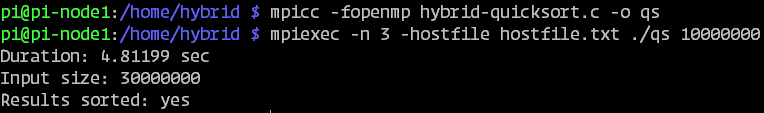
\includegraphics[width=\textwidth]{images/hybrid-sort-output.png}

\begin{exercise}
Compile \texttt{hybrid-sort.c}. Record the execution times when sorting 30 million integers with 1, 2, and 3 nodes and four OpenMP threads per node. Note that since the program's command line argument only describes the elements sorted \emph{per node}, different arguments will need to be used to sort 30 million integers total, depending on the number of nodes.
\end{exercise}
\end{document}
